{将被排序的记录数组R{[}1..n{]}垂直排列,每个记录R{[}i{]}看作是重量为R{[}i{]}.key的气泡。根据轻气泡不能在重气泡之下的原则,从下往上扫描数组R:凡扫描到违反本原则的轻气泡,就使其向上``飘浮''。如此反复进行,直到最后任何两个气泡都是轻者在上,重者在下为止。}

{~ ~ ~ 如下图所示。}

{\includegraphics[width=2.08333in,height=2.08333in]{png-jpeg-pics/e671e1d1d184b3e9b8d2b7d9dacab253.peg?}\\
\hspace*{0.333em}}

{\textbf{解释如下:}上图中的a和上图中的b分别是第一趟起泡和第二趟起泡的过程。白色和灰色的都是无序的起泡,灰色是当前向上浮动的气泡。黑色为已经有序的气泡。当向上浮动的起泡遇到比它重的气泡时,就跟大气泡交换位置。若遇到比它轻的气泡时,轻气泡就变成灰色气泡(向上浮动的气泡)。当某一轮起泡,都没有发生气泡交换位置的情况时,说明起泡排序结束。}

{\textbf{代码如下:}}{}

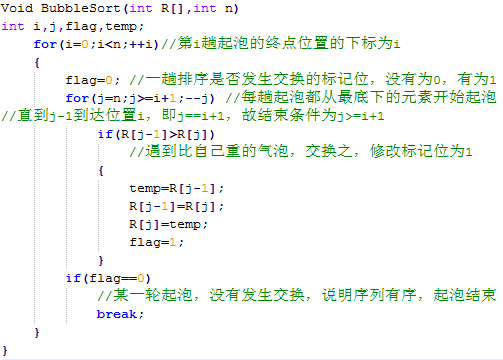
\includegraphics[width=3.70833in,height=2.65625in]{png-jpeg-pics/232C7FCF5B9C314B522DA40F90E151B7.png}

{\textbf{算法分析:}最好情况下的时间复杂度为}{O(n)}{,最坏情况下的时间复杂度为}{O(n\textsuperscript{2})}{。空间复杂度为}{O(1)}{。}
